\documentclass[a4paper, german, lecturenumbers = true, number small environments = theorem, hide version]{mkessler-script}

\course{Einführung in die Geometrie und Topologie}
\lecturer{Daniel Kasprowski}
\assistant[f]{Arunima Ray}
\author{Maximilian Keßler}

\RequirePackage{mkessler-math}
\RequirePackage{mkessler-fancythm}
\usepackage{epsfig}
%\usepackage{psfrag}
%\usepackage{sseq} (if you need to draw spectral sequences, please use this package, available at http://wwwmath.uni-muenster.de/u/tbauer/)
\usepackage{mathrsfs}
\usepackage{amscd}
\usepackage{amsbsy}
\usepackage{verbatim}
\usepackage{moreverb}

\newtheorem{prop}[theorem]{Proposition}
\newtheorem{cor}[theorem]{Corollary}
\newtheorem{conj}[theorem]{Conjecture}


\theoremstyle{definition}
\newtheorem{hw}{Homework}
\newtheorem{exercise*}[exercise]{$\star$ Exercise}

\theoremstyle{remark}
\newtheorem{aside}[theorem]{Aside}

\newcommand{\nn}{\nonumber}
\newcommand{\nid}{\noindent}
\newcommand{\ra}{\rightarrow}
\newcommand{\la}{\leftarrow}
\newcommand{\xra}{\xrightarrow}
\newcommand{\xla}{\xleftarrow}
\newcommand{\tto}{\longrightarrow}

\newcommand{\weq}{\xrightarrow{\sim}}
\newcommand{\cofib}{\rightarrowtail}
\newcommand{\fib}{\twoheadrightarrow}

\newcommand{\IRep}{\mathrm{IRep}}
\newcommand{\IHom}{\mathrm{IHom}}

\def\llarrow{   \hspace{.05cm}\mbox{\,\put(0,-2){$\leftarrow$}\put(0,2){$\leftarrow$}\hspace{.45cm}}}
\def\rrarrow{   \hspace{.05cm}\mbox{\,\put(0,-2){$\rightarrow$}\put(0,2){$\rightarrow$}\hspace{.45cm}}}
\def\lllarrow{  \hspace{.05cm}\mbox{\,\put(0,-3){$\leftarrow$}\put(0,1){$\leftarrow$}\put(0,5){$\leftarrow$}\hspace{.45cm}}}
\def\rrrarrow{  \hspace{.05cm}\mbox{\,\put(0,-3){$\rightarrow$}\put(0,1){$\rightarrow$}\put(0,5){$\rightarrow$}\hspace{.45cm}}}

\def\cA{\mathcal A}\def\cB{\mathcal B}\def\cC{\mathcal C}\def\cD{\mathcal D}
\def\cE{\mathcal E}\def\cF{\mathcal F}\def\cG{\mathcal G}\def\cH{\mathcal H}
\def\cI{\mathcal I}\def\cJ{\mathcal J}\def\cK{\mathcal K}\def\cL{\mathcal L}
\def\cM{\mathcal M}\def\cN{\mathcal N}\def\cO{\mathcal O}\def\cP{\mathcal P}
\def\cQ{\mathcal Q}\def\cR{\mathcal R}\def\cS{\mathcal S}\def\cT{\mathcal T}
\def\cU{\mathcal U}\def\cV{\mathcal V}\def\cW{\mathcal W}\def\cX{\mathcal X}
\def\cY{\mathcal Y}\def\cZ{\mathcal Z}

\def\sA{\mathscr A}\def\cB{\mathcal B}\def\cC{\mathcal C}\def\cD{\mathcal D}
\def\cE{\mathcal E}\def\cF{\mathcal F}\def\sG{\mathscr G}\def\cH{\mathcal H}
\def\cI{\mathcal I}\def\cJ{\mathcal J}\def\cK{\mathcal K}\def\cL{\mathcal L}
\def\cM{\mathcal M}\def\cN{\mathcal N}\def\cO{\mathcal O}\def\cP{\mathcal P}
\def\cQ{\mathcal Q}\def\cR{\mathcal R}\def\cS{\mathcal S}\def\cT{\mathcal T}
\def\cU{\mathcal U}\def\cV{\mathcal V}\def\cW{\mathcal W}\def\cX{\mathcal X}
\def\cY{\mathcal Y}\def\cZ{\mathcal Z}

\def\fG{\mathfrak G}\def\fH{\mathfrak H}
\def\fS{\mathfrak S}\def\fN{\mathfrak N}\def\fX{\mathfrak X}\def\fY{\mathfrak Y}

\def\op{\textrm{op}}\def\ob{\textrm{ob}}

%\def\Iso{\mathcal Iso}\def\cInn{\mathcal Inn}

\def\fg{\mathfrak g}\def\fh{\mathfrak h}\def\fri{\mathfrak i}\def\fp{\mathfrak p}
\def\fA{\mathfrak A}\def\fU{\mathfrak U}

\def\AA{\mathbb A}\def\BB{\mathbb B}\def\CC{\mathbb C}\def\DD{\mathbb D}
\def\EE{\mathbb E}\def\FF{\mathbb F}\def\GG{\mathbb G}\def\HH{\mathbb H}
\def\II{\mathbb I}\def\JJ{\mathbb J}\def\KK{\mathbb K}\def\LL{\mathbb L}
\def\MM{\mathbb M}\def\NN{\mathbb N}\def\OO{\mathbb O}\def\PP{\mathbb P}
\def\QQ{\mathbb Q}\def\RR{\mathbb R}\def\SS{\mathbb S}\def\TT{\mathbb T}
\def\UU{\mathbb U}\def\VV{\mathbb V}\def\WW{\mathbb W}\def\XX{\mathbb X}
\def\YY{\mathbb Y}\def\ZZ{\mathbb Z}

\def\TOP{\mathcal{TOP}}\def\GRP{\mathcal{GRP}}\def\GRPD{\mathcal{GRPD}} \def\CAT{\mathcal{CAT}} \def\SET{\mathcal{SET}}

\def\id{\mathrm{id}}\def\Id{\mathrm{Id}}
\def\inverse{^{-1}}



\begin{document}
    \maketitle
    \begin{abstract}
    {\color{red} Achtung:} Diese Version des Skripts benutze ich zur Bearbeitung! Einige Dinge fehlen, dafür gibt es TODO-Notes. Für Inhalte, benutzt die \href{https://kesslermaximilian.github.io/LectureNotesBonn/2021_Topologie.pdf}{normale Version}
    \end{abstract}
    \newpage
    \listoftodos
    \newpage
    \summaryoflectures
    \newpage
    % start lectures
    \setcounter{section}{19}
    \setcounter{dummy}{1}
    \setcounter{smalldummy}{0}
    \setcounter{figure}{28}
    \setcounter{claim}{1}
    \setcounter{lecture}{18}
    %! TEX root = ../../master.tex
\lecture[Decktransformationen von $\exp\colon\R -> S^1$. Normalisatoren. Gruppenisomorphismus $\Delta(p)\cong H \backslash N_{pi1(X,x0)}H$ zwischen Decktransformationen und ~Fundamentalgruppe. Gruppenwirkungen. Semidirekte Produkte und die Fundamentalgruppe des Torus $\Z \rtimes \Z$.]{Di 29 Jun 2021}{Decktransformationen}
\begin{example}
    \begin{enumerate}[1)]
        \item Betrachte wieder die Überlagerung $\exp \colon  \R \to  S^1$.
            \begin{claim*}
                $\Delta(\exp) = \left \{T_n \mid  n\in \Z\right\} $ mit $T_n(x) = x+n$.
            \end{claim*}
            \begin{proof}
                Wir zeigen zunächst, dass es sich überhaupt um Decktransformationen handelt. Offensichtlich sind das Automorphismen von $\R$, wir müssen noch zeigen, dass diese über $S^1$ sind, es ist hierzu
                 \[
                     \exp (T_n(x)) = \exp (x+n) = \exp (x)
                .\] 

                Sei nun $f\in \Delta(\exp )$ eine beliebige Decktransformation. Dann ist $f(0) \in \Z$ weil $\exp ^{-1}(1) \in \Z$ und $f$ ein Morphismus über  $S^1$ ist. Betrachte nun
                    \begin{equation*}
            \varphi \colon \left|        \begin{array}{c c l} 
                    \R & \longrightarrow & \R \\
                    x & \longmapsto &  f(x) - (x + f(0))
                    \end{array}\right.
                \end{equation*}
               Dann ist
               \[
                   \exp (f(x) - (x + f(0)) = \exp (f(x)) \cdot  \exp (x)^{-1} \cdot \exp (f(0))^{-1} = \exp (x) \exp (x)^{-1} = 1
               .\] 
               Also ist $\varphi (\R) \in \Z$, also konstant weil $\Z$ die diskrete Topologie trägt. Mit $f(0) - (0 + f(0)) = 0$ sehen wir $\varphi  \equiv 0$.
                \[
                    f(x) = x + f(0) \quad \implies \quad f = T_{f(0)}
               .\] 
               also haben wir tatsächlich alle solchen Überlagerungen gefunden.
            \end{proof}
        \item Betrachte für $n\geq 2$ die Überlagerung $p\colon  S^n \to  \R\mathbb{P}^n$.
            \begin{claim*}
                Dann ist $\Delta(p) = \left \{\id_{S^n}, ι\right\} $, wobei $ι$ die Antipodalabbildung sein sollte.
            \end{claim*}
            \begin{proof}
                Es ist klar, dass die beiden vorgegebenen Abbildungen Decktransformationen sind.

                Ist $f\in \Delta(p)$, so ist bereits $f(x) = \sgn(x) \cdot x$, wobei
                \[
                \sgn \colon  S^n \to  \left \{-1,1\right\} 
                .\] 
                stetig ist. Die Abbildung $\sgn$ ist also konstant, und es folgt  $f=\id_{S^n}$ für $\sgn \equiv 1$, und $f = ι$ für  $\sgn \equiv -1$.
            \end{proof}

            Also ist $\Delta(p) \cong \Z / 2\Z$, denn es gibt nur eine Gruppe mit 2 Elementen.
    \end{enumerate}
\end{example}
\todo{Buchstabe für die Antipodalabbildung?}

\begin{notation*}
    Ist $H$ eine Untergruppe von  $G$, so schreiben wir  $H \leq G$, nicht wie ansonsten üblich $H \subset G$.
\end{notation*}

\begin{definition}[Normalisator]\label{def:normalisator}
    Sei $H\leq  G$ eine Untergruppe. Der \vocab{Normalisator} von $H$ in  $G$ ist definiert durch
    \[
    N_GH \coloneqq  \left \{g\in G \mid  gH g^{-1} = H\right\} 
    .\] 
    Diest ist eine Untergruppe von $G$.
\end{definition}

\begin{remark*}
    Der Begriff Normalisator kommt daher, dass es sich bei $N_GH$ um die größte Untergruppe von  $G$ handelt, in der  $H$ noch normal ist. Ist  $H$ ein Normalteiler von  $G$, so ergibt sich  $N_GH = G$. Außerdem erkennt man so, dass auch  $H \leq  N_GH$.
\end{remark*}

\begin{remark}
    Die Bedingung $gH g^{-1} = H$ sagt \textit{nicht} notwendigerweise aus, dass $ghg^{-1} = h$ für $h\in H$, nur dass die beiden entstehenden Mengen gleich sind.    
\end{remark}

\begin{remark}
    Per Definition ist $H$ normal in  $N_GH$. Also ist $H \backslash N_GH$ (die Menge der Linksnebenklassen) wieder eine Gruppe mittels
    \[
        (Hg) (Hg') = H(gg')
    .\] 
\end{remark}

\begin{oral}
    Es gibt erstmal keinen Grund, warum wir die \textit{Links}nebenklassen verwenden, für die Rechtsnebenklassen gilt Obiges auch. Wir werden aber später im Zusammenhang mit Gruppentheorie sehen, dass es aus Konsistenzgründen besser ist, jetzt schon mit Linksnebenklassen zu arbeiten, damit wir später nicht zwischen den beiden Konzepten wechseln müssen.
\end{oral}

\underline{Erinnerung} Ist $p\colon  E\to X$ eine Überlagerung mit $X$ zusammenhängend und lokal wegzusammenhängend,  $x_0\in X$ und $e_0\in p^{-1} (x_0)$ sowie $H\coloneqq p_*(\pi_1(E,e_0))$ die charakteristischen Untergruppe. Dann ist
    \begin{equation*}
    \varphi : \left| \begin{array}{c c l} 
        E & \longrightarrow & \left \{\text{Weg $w$ in  $X$}\mid  w(0) = x_0\right\} / \text{$H$-Äquivalenz} \\
e & \longmapsto &  \left[ p \circ  v \right] _H
    \end{array} \right.
\end{equation*}
eine Bijektion, wobei $v$ ein Weg von  $e_0$ nach $e$ sei.
\todo{Erklärung davon}

Insbesondere erhalten wir auch eine Bijektion
\[
    \varphi (p^{-1} (x_0)) = \faktor{\pi_1(X,x_0)}{\text{$H$-Äquivalenz}}
.\] 

\begin{restatable}{theorem}{ThmDecktransformationNormalisator}\label{thm:isomorphismus-von-decktransformationen-mit-nebenklassengruppe-von-charakteristischer-untergruppe-in-seinem-normalisator}
    Seien $E,X,p,x_0,e_0,H$ wie oben.
    \begin{enumerate}[1)]
        \item Für $f\in \Delta(p)$ ist
            \[
                \varphi (f(e_0)) \in H \backslash N_{\pi_1(X,x_0)}H
            .\] 
        \item Die Abbildung
                \begin{equation*}
                \psi : \left| \begin{array}{c c l} 
                    \Delta(p) & \longrightarrow & H \backslash N_{\pi_1(X,x_0)}H \\
                    f & \longmapsto &  \varphi (f(e_0))
                \end{array} \right.
            \end{equation*}
           ist ein Gruppenisomorphismus. 
    \end{enumerate}
\end{restatable}

\begin{dcorollary}\label{cor:bei-universeller-überlagerung-sind-decktransformationen-isomorph-zu-fundamentalgruppe}
    Ist $p$ die universelle Überlagerung von  $X$, so ist
    \[
        \Delta(p) \cong \pi_1(X,x_0)
    .\] 
\end{dcorollary}

\begin{proof}
    Ist $p$ die universelle Überlagerung, so ist  $H = p_*(\pi_1(E,e_0)) = \left \{1\right\} $ die triviale Untergruppe, d.h. $N_{\pi_1(X,x_0)}H = \pi_1(X,x_0)$.
\end{proof}

\begin{proof}[Beweis von \autoref{thm:isomorphismus-von-decktransformationen-mit-nebenklassengruppe-von-charakteristischer-untergruppe-in-seinem-normalisator}]
    \begin{enumerate}[1)]
        \item Es ist $f$ eine Hebung von  $p$, denn es kommutiert ja
            \[
             \begin{tikzcd}
                & E \ar{d}{p} \\
                 E \ar{ur}{f} \ar[swap]{r}{p} & X
            \end{tikzcd}
        \]
    Nach dem \nameref{thm:allgemeiner-liftungssatz} ergibt sich nun
    \[
        H = p_*(\pi_1(E,e)) \leq  p_*(\pi_1(E,f(e_0))
    .\] 
    Sei $v$ ein Weg von  $e_0$ zu $f(e_0)$. Dann ist
    \[
        H\leq p_*(\pi_1(E,f(e_0)) = [p \circ  v] ^{-1} \star p_*(\pi_1(E,e_0)) \star [p \circ  v]
    .\]
    Also ergibt sich zusammen
    \[
        [p \circ  v] ^{-1} \star H \star [p \circ  v] \leq H
    .\] 
    Vertauschen von $e_0,f(e_0)$ sowie Ersetzung von $f$ durch  $f^{-1}$ ergibt nun, dass auch
    \[
        [p \circ  v] \star H \star [p \circ v] ^{-1} \leq H
    .\] 
    und aus Symmetrie folgt dann
    \[
        [p \circ  v] \star H \star [p \circ  v] ^{-1} = H
    .\] 
    also folgt $[p \circ v] \in N_{\pi_1(X,x_0)} H$, und somit insbesondere
    \[
        \varphi (f(e_0)) = [p \circ  v]_H \in H \backslash N_{\pi_1(X,x_0)} H
    .\] 
\item
    \begin{description}
        \item[Injektivität] Seien $f,g \in \Delta(p)$ mit
            \[
                \varphi (f(e_0)) f \psi (f) = \psi (g) = \varphi (g(e_0))
            .\] 
            so folgt aus Injektivität von $\varphi $ zunächst $f(e_0) = g(e_0)$, aber $f,g$ sind Hebungen von  $p$ und stimmen in  $e_0$ überein, also gilt $f=g$ nach der Eindeutigkeit im  \nameref{thm:allgemeiner-liftungssatz}.
        \item[Surjektivität] Sei $[w] \in N_{\pi_1(X,x_0)}H$ ein Element aus dem Normalisator. Sei $e_0' \coloneqq  L(w,e_0)(1)$ der Endpunkt der Hebung von $e_0'$.

            Es ist nach \autoref{thm:charakteristische-untergruppen-innerhalb-der-faser-sind-nur-konjugiert-wenn-weg-zwischen-urbildern-existiert} nun:
            \begin{IEEEeqnarray*}{rCl}
                p_*(\pi_1(E,e_0')) & = & [\underbrace{p \circ  L(w,e_0)}_{=w^{-1}}]^{-1}\star H \star [\underbrace{p \circ  L(w,e_0)}_{= w}] \\
                                  & \stackrel{[w]\in N_{\pi_1(X,x_0)}H}{=}  & H
            \end{IEEEeqnarray*}
            Nach \autoref{thm:äquivalenz-von-überlagerungen-über-lokal-wegzsuammenhängendem-wegzusammenhängendem-raum} gibt es also einen Homöomorphismus $f\colon  E \stackrel{\cong}{\longrightarrow} E$ mit $p \circ  f = p$ und $f(e_0) = e_0'$, bei $f$ handelt es sich dann um eine Decktransformation, und wir sehen leicht
             \[
                 \psi (f) = \varphi (f(e_0)) = \varphi (e_0') = [p \circ  L(w,e_0)]_H = [w]_H
            .\] 
        \item[Gruppenhomomorphismus]
            Seien $f,g \in \Delta(p)$ und $v$ ein Weg von  $e_0$ nach $f(e_0)$ sowie $v'$ ein Weg von  $e_0$ nach $g(e_0)$. Dann ist $g \circ v$ ein Weg von $g(e_0)$ nach $g(f(e_0))$ und $v' \star (g \circ v)$ ein Weg von $e_0$ nach $g(f(e_0))$.

            Es ist nun
            \begin{IEEEeqnarray*}{rCl}
                \psi (g \circ f) & = & [p \circ  (v\star (g \circ v))]_H \\
                                 & = & H[p \circ  (v' \star (g \circ v))] \\
                                 & = & H[(p \circ  v') \star p(g \circ v)] \\
                                 & = & H[p\circ v')] \star H[p (g \circ v)] \\
                                 & \stackrel{p \circ  g = p}{=}  & H[p \circ v'] \star H[p \circ v] \\
                                 & = & \psi (g) \star \psi (f)
            \end{IEEEeqnarray*}
    \end{description}
    \end{enumerate}
\end{proof}

\begin{remark*}
    Hier kam in der Vorlesung etwas zu Gruppen und Nebenklassen etc. Das wird noch nachgeholt, ich war mit Links- / Rechtsnebenklassen und deren Bezeichnung selbst etwas verwirrt.
\end{remark*}


\begin{definition}[$G$-Menge]\label{def:g-menge}
    Sei $G$ eine Gruppe. Eine \vocab[$G$-Menge]{(Rechts-) $G$-Menge} ist eine Menge  $X$ mit einer Abbildung
        \begin{equation*}
        .: \left| \begin{array}{c c l} 
        X\times G & \longrightarrow & X \\
        (x,g) & \longmapsto &  x.g
        \end{array} \right.
    \end{equation*}
    für die gilt
    \begin{enumerate}[i)]
        \item $x.1 = x$ für  $x\in X$
        \item $(x.g).h = x.(gh)$ für  $x\in X$ und $g,h\in G$.
    \end{enumerate}
    Ein \vocab{Homomorphismus von $G$-Mengen} ist eine Abbildung $f\colon X \to  Y$, so dass
\[
    f(x.g) = f(x).g \qquad \forall x\in X, g\in G
.\] 
\end{definition}

\begin{remark}[Ent- oder auch Verwirrung bezüglich Rinks und Lechts]
    Analoges können wir für links-$G$-Mengen definieren, dann fordern wir  $h.(g.x) = (hg).x$. Eine Links- $G$-menge ist eine Rechts-$G$-Menge mittels
     \[
    x.g \coloneqq g^{-1}x.
    .\] 
    bzw. wir können auch eine Links-$G$-Menge als Rechts-$G^{\op}$-Menge auffassen.

Eine Links-$G$-Menge ist nämlich nichts anderes als Ein Funktor  $\mathcat{G} \to  \Set$, und eine Rechts-$G$-Menge ist ein Funktor  $\mathcat{G}^{\op} \to  \Set$, aber wegen $\mathcat{G} \cong \mathcat{G}^{\op}$ sind die Konzepte äquivalent.
\end{remark}

\begin{trivial}
    $G$-Mengen sind also genau Funktoren  $\mathcat{G} \to  \Set$, und Morphismen von $G$-Mengen  $X,Y \colon  \mathcat{G} \to  \Set$ sind genau natürliche Transformationen $X \to Y$.

    Die Kategorie der $G$-Mengen über einer Gruppe  $G$ ist dann genau die Funktorkategorie  $[\mathcat{G},\Set]$.
\end{trivial}

\begin{example}
    Ist $H\leq G$, so ist $H \backslash G$ eine  $G$-Menge mittels  $(Hg)g' = H(gg')$.
\end{example}

\begin{nexample}\label{ex:fundamentalgruppe-der-kleinschen-flasche-mittels-semidirektem-produkt-z-z}
    Das semidirekte Produkt $\Z \rtimes Z$ von $\Z$ mit $\Z$ ist die Gruppe mit Menge $\Z\times \Z$ und Verknüpfung
    \[
        (n,m)(n',m') = (n+(-1)^m n', m + m')
    .\] 
    Es gibt eine Rechtswirkung
        \begin{equation*}
        \begin{array}{c c l} 
            \R^2\times (\Z\rtimes \Z) & \longrightarrow & \R^2 \\
            ((x,y),(n,m)) & \longmapsto &  ((-1)^m(x+n),y+m)
        \end{array}
    \end{equation*}
    (Übung, dass das die Axiome erfüllt).
    \begin{claim*}
        $\forall (x,y) \in \R^2 \; \exists (n,m) \in \Z\rtimes \Z$, sodass
        \[
            (x,y).(n.m) \in I^2
        .\] 
    \end{claim*}
    \begin{proof}
        Sei $(x,y) \in \R^2$ beliebig. Zunächst existiert ein $m\in \Z$, sodass $y + m \in I$, und dann existiert ein $n\in \Z$ mit $(-1)^m x + n\in I$, dann ist
        \[
            (x,y) . \underbrace{(0,m).(n,0)}_{=((-1)^mn, m)} = ((-1)^mx, y+m)(n,0) = ((-1)^mx + n, y+m)
        .\] 
    \end{proof}
        Falls $x\not\in \Z, y\not\in \Z$, so sind $n,m$ eindeutig bestimmt. Mittels den Gleichungen
        \[
            (t,0).(0,1) = (-t,1) \qquad (0,t).(1,0) = (1,t)
        .\] 
        folgt nun, dass $\faktor{\R^2}{(\Z \rtimes \Z)}$ die Kleinsche Flasche ist.
        \begin{claim*}
            Die Abbildung $\R^2 \to  \faktor{\R^2}{\Z \rtimes \Z}$ ist eine Überlagerung und $\Z \rtimes \Z$ sind die Decktransformationen.
        \end{claim*}
        \begin{proof}
            Übung.
        \end{proof}
        Da $\R^2$ einfach zusammenhängend ist, folgt mit \autoref{cor:bei-universeller-überlagerung-sind-decktransformationen-isomorph-zu-fundamentalgruppe}, dass
        \[
            \pi_1(K) \cong \Z \rtimes \Z
        .\] 
\end{nexample}

\begin{oral}
    Semidirekte Produkte machen zwischen beliebigen Gruppen $G, H$ sind, wenn wir eine Wirkung von $G$ auf  $H$ haben. In obigem Fall gibt es aber nur eine nichttriviale Wirkung von  $\Z$ auf $\Z$, weswegn wir von \textit{dem} semidirekten Produkt $\Z \rtimes \Z$ sprechen können. 
\end{oral}

    %! TEX root = ../../master.tex
\lecture[Transitive Gruppenwirkungen. Orbit, Stabilisator. Zerlegung von Gruppenwirkungen in Orbite, Isomorphismus mit den Stabilisatornebenklassen. Hauptsatz der Überlagerungstheorie.]{Do 01 Jul 2021}{Hauptsatz der Überlagerungstheorie}

Wir starten mit einem Überblick der letzten Vorlesungen:
\restatetheorem*{AllgemeinerLiftungssatz}

\restatetheorem*{DefCharakteristischeUntergruppe}

\restatetheorem*{ThmHomoeomorpheUeberlagerungen}

\restatetheorem*{ThmKonjugierteCharakteristischeUntergruppen}

\restatetheorem*{ThmUniverselleUeberlagerung}

Insgesamt können wir folgendes zusammenfassen:

\[
    \faktor{\text{zsh. Überlagerungen von $X$}}{\text{Hom über $X$ }} \stackrel{1:1}{\leftrightarrow} \left \{\parbox{14em}{Konjugationsklassen von Untergruppen in $\pi_1(X,x_0)$}\right\} 
\]

\begin{oral}
    Das ganze ist schon sehr toll, aber bisher 'nur' eine mengentheoretische Aussage. Wir würden gerne auch die Homomorphismen (nicht-Isomorphismen insbesondere, die Isomorphismen verstehen wir, zumindest deren Existenz) verstehen.

    Der Hauptsatz der Überlagerungstheorie verfolgt genau dieses Ziel, er gibt eine kategorientheoritschere Verallgemeinerung von obiger Bijektion.
\end{oral}

\begin{definition}
    Eine $G$-Menge  $X$ heißt  \vocab{transitiv}, falls $\forall x,y \in X$ $\exists g\in G$ mit $x.g = y$. 
\end{definition}

\begin{dnotation}
   Wir sagen auch, dass die Wirkung von $G$ auf  $X$ transitiv ist. 
\end{dnotation}

\begin{example}
    Sei $H\subset G$ eine Untergruppe. Dann ist $\cofaktor{H}{G}$, die Menge der Nebenklassen von  $H$, eine transitive  $G$-Menge. Für  $Hg, Hg' \in  \cofaktor{H}{G}$ haben wir nämlich die Wirkung $Hg.(g^{-1}g') = Hg'$.
\end{example}

\begin{lemmadef}[Bahn]\label{def:bahn-orbit}
    Sei $X$ eine  $G$-Menge und  $x\in X$. Dann definiert
    \[
    x.G = \left \{x.g \mid  g\in G\right\} 
    .\] 
    die \vocab{Bahn} oder auch \vocab{Orbit} von $x$. Dann ist  $x.G$ eine Unter- $G$-Menge und  $x.G$ ist transitiv.
\end{lemmadef}
\begin{proof}
    \begin{description}
        \item[Abgeschlossenheit] Sei $x.g \in x.G$ beliebig, dann ist die Wirkung unter einem beliebigen $g'$ genau
            \[
                (x.g).g' = x.(g \circ g')
            .\] 
            in $x.G$ enthalten, weil  $g \circ  g'\in G$.
        \item[Transitivität] Seien $x.g$ und  $x.g'\in x.G$ beliebig. Dann ist
            \[
                (x.g).(gg^{-1}) = x.(gg^{-1}g') = x.g'
            .\] 
            und somit ist die Wirkung transitiv.
    \end{description}
\end{proof}

\begin{lemma}
Sei $X$ eine  $G$-Menge. Seien $x,x' \in X$ beliebig. Dann ist $x.G = x'.G$ oder  $(x.G) \cap  (x'.G) = \emptyset$.
\end{lemma}

\begin{proof}
    Nimm an, dass $(x.G) \cap  (x'.G) \neq  \emptyset$. Wähle also ein $y$ mit 
     \[
         y\in  (x.G) \cap  (x'.G)
    .\] 
    Dann ist also $y = x.g = x'.g'$ für  $g,g' \in G$. Dann ist aber für alle $h\in G$ auch
    \[
        x.h = x.(g.g^{-1}).h = (x.g).g^{-1}.h = y.g^{-1}.h = x'.(g'g^{-1}h) \in x'G
    .\] 
    also ergibt sich $x.G \subset x'G$. Aus Symmetrie folgt $x'.G \subset x.G$, also sind die Klassen gleich.
\end{proof}

\begin{dcorollary}\label{cor:g-menge-ist-disjunkte-vereinigung-der-bahnen}
    Jede $G$-Menge ist die disjunkte Vereinigung ihrer Bahnen.
\end{dcorollary}

\begin{dlemmadef}[Stabilisator]\label{def:stabilisator}
    Sei $X$ eine  $G$-Menge und  $x\in X$. Dann ist der \vocab{Stabilisator} von $x$ die Untergruppe
    \[
    G_x = \left \{g\in G \mid  x.g = x\right\}\leq  G
    .\] 
\end{dlemmadef}
\begin{proof}
    Ist $g\in G_x$, so ergibt sich
    \[
        x = x.e = x.(gg^{-1}) = x.g.g^{-1} = x.g^{-1}
    .\] 
    also ist auch $g^{-1}\in G_x$. Sind zudem $g,h\in G_x$ beliebig, so erhalten wir mit
    \[
        x.(gh) = x.g.h = x.h = x
    .\] 
    auch sofort, dass $gh \in G_x$. Also ist $g_x \leq  G$ tatsächlich eine Untergruppe wie behauptet.
\end{proof}

\begin{lemma}
    Sei $X$ eine  $G$-Menge und  $x\in X$. Dann ist $x.G$ isomorph (als  $G$-Menge) zu  $\cofaktor{G_x}{G}$.
\end{lemma}
\begin{proof}
    Definiere
        \begin{equation*}
        \varphi : \left| \begin{array}{c c l} 
            \cofaktor{G_x}{G} & \longrightarrow & x.G \\
        G_xg & \longmapsto &  x.g
        \end{array} \right.
    \end{equation*}
    \begin{description}
        \item[Wohldefiniertheit] Gleiche Elemente auf der linken Seite unterscheiden sich in ihrer Darstellung nur um ein Element aus $h\in G_x$, wir wollen zeigen, dass dies gleiches Bild ergibt:
            \[
                \varphi (G_xhg) = x.(hg) = x.h.g = x.g = \varphi (G_xg)
            .\] 
        \item[Injektivität] Ist $x.g = x.g'$, dann ergibt sich auch
             \[
            x = x.g'.g^{-1}
            .\] 
            und daraus folgt bereits, dass $g'g^{-1} \in G_x$ nach Definition, also
            \[
                G_xg = G_xg'(g^{-1}g) = G_x(\underbrace{g'g^{-1}}_{\in G_x})g = G_xg'
            .\] 
            also waren auch schon die Nebenklassen gleich.
        \item[Surjektivität] Ist $x.g\in x.G$ beliebig, so ist offensichtlich
            \[
                x.g = \varphi (G_xg)
            .\] 
        \item[$G$-Äquivarianz] (Homomorphismus von $G$-Mengen). Es ist
             \[
                 \varphi ((G_xg)g') = \varphi (G_x(gg')) = x.(gg') = (x.g).g' = \varphi (G_xg).g'
            .\] 
    \end{description}
    Die Mengentheoretische Umkehrabbildung ist dann auch $G$-Äquivariant, also ist  $\varphi $ ein Isomorphismus.
\end{proof}

    \begin{oral}
        Auch, wenn das im Allgemeinen nicht so ist, dass Mengentheorischer Isomorphismus + Kategorientheoretischer Homomorphismus $\implies$ Kategorieller Isomorphismus (das gilt ja z.B. in $\Top$ nicht, siehe  $\exp \colon  [0,1) \to  S^1$), gilt dies für $G$-Mengen (und im Übrigen auch für Gruppen).
    \end{oral}

    Also ist jede $G$-menge isomorph zu einer disjunkten Vereinigung um $G$-Mengen der Form $\cofaktor{H}{G}$, wobei  $H\leq G$.

\begin{warning}
    Auch, wenn wir die Notation $\cofaktor{H}{G}$ verwendet haben, wollen wir damit nicht notwendigerweise ausdrücken, dass  $H$ normal ist in  $G$, wir haben nur die Menge der Nebenklassen betrachtet, und zwar als Menge.
\end{warning}

\section{Hauptsatz der Überlagerungstheorie}

Sei in diesem Kapitel stets $p\colon  E\to X$ eine Überlagerung.

\begin{lemmadef}
    Die Gruppe $\pi_1(X,x_0)$ wirkt folgendermaßen auf $p^{-1} (x_0)$: Sei $e\in p^{-1} (x_0)$, und $[w]\in \pi_1(X,x_0)$, dann definiere
    \[
        e.[w] = L(w,e)(1) \in p^{-1} (x_0)
    .\] 
    Mit dieser Wirkung ist $p^{-1} (x_0)$ eine $G$-Menge.
\end{lemmadef}
\begin{proof}
    \begin{description}
        \item[Wohldefiniertheit] Sind $w,w'$ homotop relativ Endpunkten sind, dann auch  $L(w,e)$ und  $L(w',e)$ nach dem \nameref{thm:homotopieliftungssatz}, also sind insbesondere ihre Endpunkte gleich.
        \item[Axiome der Gruppenwirkung] Es ist offenbar
            \[
                e.[c_{x_0}] = L(c_{x_0},e) = c_{e}(1) = e
            .\] 
            und auch 
            \begin{IEEEeqnarray*}{rCl}
                e.([w] \star [w]) & = & L(w \star w,e)(1) \\
                                  & = & (L(w,e)\star L(w',L(w,e)(1)))(1) \\
                                  & = & L(w',\underbrace{L(w,e(1)}_{= e.[w]})(1) \\
                                  & = & (e.[w]).[w']
            \end{IEEEeqnarray*}
    \end{description}
\end{proof}

\begin{oral}
    An dieser Stelle geht das einzige Mal ein, dass wir links-$G$-Mengen betrachtet haben, weil wir die Verknüpfung von Schleifen in dieser Richtung definiert hatten.
\end{oral}

\begin{lemma}
    Sind $p\colon  E\to X$ und $p'\colon E'\to X$ Überlagerungen sowie $x_0\in X$. Sei $f\colon  E\to  E'$ eine Abbbildung von Überlagerungen, d.h. $p = p' \circ f$. Dann ist
    \[
        f|_{p^{-1} (x_0)}\colon  p^{-1} (x_0) \to  p'^{-1}(x_0)
    .\] 
    ein Homomorpismus von $\pi_1(X,x_0)$-Mengen.
\end{lemma}
\begin{proof}
    \begin{description}
        \item[Wohldefiniertheit] Sei $e\in p^{-1} (x_0)$. Dann ist $p'(f(e)) = p(e) = x_0$, also ist $f(e) \in p^{-1} (x_0)$.
        \item[Äquivarianz] Sei $e\in p^{-1} (x_0)$ sowie $[w]\in \pi_1(X,x_0)$ beliebig. Dann ist
            \[
                f(e).[w] = L_{p'}(w,f(e))(1) \stackrel{!}{=} f \circ L_p(w,e)(1) = f(e.[w])
            .\] 
            Das ergibt sich aber, indem wir nachrechnen, dass $f \circ  L_p(w,e)$ \textit{eine} Liftung ist, denn
            \[
                p' \circ  f \circ  L_p(w,e) = p \circ  L_p(w,e) = w
            .\]
            aber mittlerweile ist uns klar, dass Liftungen eindeutig sind nach dem \nameref{thm:weghebungssatz}.
    \end{description}
\end{proof}

\begin{lemma}\label{lm:funktor-von-überlagerungen-in-pi-1-mengen}
    Die Zuordnung
    \begin{IEEEeqnarray*}{cCc}
        \text{Überlagerungen von $X$} &\longrightarrow &\pi_1(X,x_0)\text{-Mengen} \\ \\
    \begin{tikzcd}
        E \ar{d}{p} \\ X
    \end{tikzcd}
    \qquad&    \longmapsto  & \qquad p^{-1} (x_0) \\ \\
    \begin{tikzcd}[column sep = tiny]
    E \ar{rr}{f} \ar[swap]{dr}{p} & & E' \ar{dl}{p'} \\
    & X
\end{tikzcd} \qquad & \longmapsto &  \qquad     f|_{p^{-1} (x_0)}: p^{-1} (x_0) \to  p'^{-1}(x_0)
    \end{IEEEeqnarray*}
    ist ein Funktor.
\end{lemma}
\begin{proof}
    Wir haben schon gezeigt, dass das eine Wohldefinierte Zuordnung (Abbildung) ist. Wir müssen noch zeigen, dass das ganze mit Verknüpfung verträglich ist, und Identitäten auf Identitäten gehen. Ist also
    \[
    \begin{tikzcd}[column sep = tiny]
    E' \ar{rr}{g} \ar[swap]{dr}{p'} & & E'' \ar{dl}{p''} \\
    & X
    \end{tikzcd}
    \]
    ein weiterer Morphismun von Überlagerungen, so ist
    \[
        (g \circ f)|_{p^{-1} (x_0)} = g|_{p^{-1} (x_0)}  \circ  f|_{p^{-1} (x_0)}
    .\] 
    und es ist sicherlich auch
    \[
        (\id_E)|_{p^{-1} (x_0)} = \id_{p^{-1}(x_0)}
    .\] 
    also erfüllt diese Abbildung die Eigenschaften eines Funktors.
\end{proof}


\begin{restatable}[Hauptsatz der Überlagerungstheorie]{theorem}{ThmHauptsatzUeberlagerungstheorie}\label{thm:hauptsatz-der-überlagerungstheorie}
    Sei $X$ zusammenhängend, lokal wegzusammenhängend, semilokal einfachzusammenhängend sowie  $x_0\in X$. Dann ist der Funktor aus \autoref{lm:funktor-von-überlagerungen-in-pi-1-mengen} eine Äquivalenz von Kategorien. Das heißt:
    \begin{enumerate}[1)]
        \item Für jede $\pi_1(X,x_0)$-Menge $M$ gibt es eine Überlagerung  $p\colon  E \to X$, so dass $p^{-1} (x_0)$ isomorph ist (als $\pi_1(X,x_0)$-Menge) zu  $M$. (\textit{essentielle Surjektivität})
        \item Für zwei Überlagerungen $p\colon  E \to X$ und $p' \colon  E' \to  X$ ist die Zuordnung
            \begin{IEEEeqnarray*}{cCc}
                \left\{
                    \begin{tikzcd}[column sep = tiny, ampersand replacement = \&]
                E \ar{rr}{f} \ar[swap]{dr}{p} \& \& E' \ar{dl}{p'} \\
                \& X
        \end{tikzcd}\right\} & \longmapsto & \left \{f|_{p^{-1} (x_0)\colon  p^{-1} (x_0) \to  p'^{-1}(x_0)}\right\} 
            \end{IEEEeqnarray*}
    \end{enumerate}
\end{restatable}

\begin{oral}
    Für die 'Entpackung' dieser kategorientheoretischen Aussage haben wir die Charakterisierung von TODO.
\end{oral}

\begin{remark}
    Die Eigenschaft, dass $X$ semilokal einfachzusammenhängend ist, benötigen wir nur für Eigenschaft 1), um z.B. eine universelle Überlagerung konstruieren zu können. Für 2) genügt es allerdings zu fordern, dass  $X$ zusammenhängend und lokal wegzusammenhängend ist.
\end{remark}

\begin{remark*}
    An dieser Stelle haben wir nun \nameref{thm:seifert-van-kampen} eingeführt, und weite Teile von \autoref{sec:seifert-van-kampen} vorgezogen, damit diese vor der Klausur bekannt sind. Erst danach sind wir hierher zurückgekommen, und haben den \nameref{thm:hauptsatz-der-überlagerungstheorie} bewiesen. 
\end{remark*}

\lecture[Bijektion zwischen Orbits und Wegekomponenten. Morphismen von transitiven $g$-Mengen. Alternativer Beweis des Isomorphismus  $\Delta(p) \cong \cofaktor{H}{N_{\pi_1(X,x_0)}H}$.]{Do 08 Jul 2021}[22]{Beweis des Hauptsatzes der Überlagerungstheorie}

Wir erinnerns uns daran, dass die Wirkung von $\pi_1(X,x_0)$ auf $p^{-1} (x_0)$ durch
\[
    e.[w] \coloneqq  L(w,e)(1)
.\] 
gegeben ist.

\begin{proposition}\label{prop:wegekomponenten-von-überlagerungsraum-sind-bahnen-von-faser-bezüglich-fundamentalgruppe-wenn-basisraum-wegzusammenhängend}
    Sei $p\colon E\to X$ eine Überlagerung,  $X$ wegzusammenhängend sowie  $x_0\in X$. Dann induziert die Inklusion $p^{-1} (x_0) \hookrightarrow E$ eine Bijektion
    \[
        \left \{\pi_1(X,x_0) - \text{Bahnen von } p^{-1} (x_0) \right\}  \stackrel{1:1}{\longleftrightarrow} \left \{\text{Wegekomponenten von } E\right\} 
    .\] 
\end{proposition}

\begin{proof}
    \begin{description}
        \item[Wohldefiniertheit] Zu zeigen: Für $e\in p^{-1} (x_0)$ liegen $e$ und  $e.[w]$ in der gleichen Wegekomponente. Es ist aber
             \[
                 e.[w] = L(w,e)(1)
            .\] 
            und damit ist $L(w,e)$ ein Weg von  $e$ nach  $e.[w]$, und somit liegen die Punkte in der gleichen Wegekomponenten von  $E$.
        \item[Injektivität] Seien  $e,e'\in p^{-1} (x_0)$, so dass diese auf die gleiche Wegkomponenten abgebildet werden, dann gibt es einen Weg $v$ von  $e$ nach  $e'$. Dann ist
             \[
                 e.\underbrace{[p \circ  v]}_{\in \pi_1(X,x_0)}  = L(p \circ  v, e)(1) = v(1) = e'
            .\] 
            also liegen $e,e'$ in der gleichen Bahn.
        \item[Surjektivität] Sei  $\tilde{E}$ eine Wegekomponente von $E$ sowie  $e\in \tilde{E}$. Aufgrund des Wegzusammenhangs von $X$ finden wir einen Weg  $v$ von  $p(e)$ nach  $x_0$. Dann ist $L(v,e)$ ein Weg von  $e$ mit Endpunkt in  $p^{-1} (x_0)$, also $\tilde{E} \cap  p^{-1} (x_0) \neq  \emptyset$.
    \end{description}
\end{proof}

Ist $e\in p^{-1} (x_0)$, so ist der Orbit
\[
    e.\pi_1(x,x_0) \cong_{\pi_1(X,x_0)-\text{Menge}} \cofaktor{\pi_1(X,x_0)_e}{\pi_1(X,x_0)}
.\] 

Also interessieren wir uns auch für Elemente aus dem Stabilisator $\pi_1(x,x_0)_e$. Hierzu ist
\[
    e.[w] = e \iff  L(w,e)(1) = e \iff  L(w,e) \text{ ist Schleife an } e \iff  [w] \in  p_*(\pi_1(E,e))
.\] 

Also ist $e.\pi_1(X,x_0) \cong \cofaktor{p_*(\pi_1(E,e))}{\pi_1(X,x_0)}$.

\begin{proof}[Beweis von \autoref{thm:hauptsatz-der-überlagerungstheorie}]
    \underline{1. Schritt} Wir zeigen die essentielle Surjektivität. Sei $M$ eine  $\pi_1(X,x_0)$-Menge. Dann ist $M$ isomorph zu einer disjunkten Vereinigung
    \[
        M = \bigsqcup_{i\in I} \cofaktor{H_i}{\pi_1(X,x_0)}
    .\] 
    Mit $H_i \leq  \pi_1(X,x_0)$. Nach \autoref{thm:universelle-überlagerungen-existieren-genau-für-semilokal-einfachzusammenhängende-lokal-wegzusammenhängenden-zusammenhängende-räume} existieren Räume $E(H_i)$, sodass
     \[
         p(H_i) \colon  E(H_i) \to  X
    .\] 
    sowie $e_i\in p(H_i)^{-1}(x_0)$ mit 
    \[
        p(H_i)_* \pi_1(E(H_i),e_i) = H_i
    .\] 
    Dann ist $p(H_i)^{-1}(x_0)$ isomorph zu $\cofaktor{H_i}{\pi_1(X,x_0)}$ nach \autoref{prop:wegekomponenten-von-überlagerungsraum-sind-bahnen-von-faser-bezüglich-fundamentalgruppe-wenn-basisraum-wegzusammenhängend} und der Vorüberlegung. Wir betrachten nun die disjunkte Vereinigung
    \[
        p\coloneqq  \coprod p(H_i) \colon  \coprod _{i \in I} E(H_i) \to  X
    .\] 
    so ist
    \[
        p^{-1} (x_0) = \bigsqcup p(H_i)^{-1}(x_0) \cong \coprod_{i \in I} \cofaktor{H_i}{\pi_1(X,x_0)} \cong M
    .\] 
    \begin{remark}
        Es fehlt noch zu zeigen, dass $p$ überhaupt eine Überlagerung ist, im allgemeinen ist das Koprodukt von Überlagerungen nämlich \textit{nicht} zwingend wieder eine Überlagerung. Wir müssen das also in diesem konkreten Fall noch zeigen.
    \end{remark}
    \begin{claim}
        Sei $x\in X$ und $x\in U\subset X$ eine wegzusammenhängende Umgebung mit $\pi_1(U) \to  \pi_1(X)$ trivial. Dann ist $U$ eine trivialisierende Umgebung für alle  $p(H_i)$ und damit auch für  $p$.
    \end{claim}
    \begin{subproof}
        Folgt unmittelbar aus der Konstruktion, die wir gewählt hatten, denn wir haben gezeigt, dass die trivialisierenden Umgebungen genau diejenigen Basiselement von $X$ aus  \autoref{lm:basis-vonsemilokal-einfachzusammenhängendem-zusammenhängendem-raum} sind, und diese waren unabhängig von der Überlagerung.
    \end{subproof}
    \underline{2. Schritt} Wir zeigen die volltreue.

    \underline{Injektivität} Seien $f,\hat{f}$ zweie Überlagerungsabbildungen, d.h.
    \[
    \begin{tikzcd}[column sep = tiny]
        E \ar{rr}{f}[swap]{\hat{f}} \ar[swap]{dr}{p} & & E' \ar{dl}{p'} \\
    & X
    \end{tikzcd}
    \]
    die unter dem Funktor das gleiche Bild haben, d.h. $f|_{p^{-1} (x_0)} = \hat{f}|_{p^{-1} (x_0)}$. Wir wollen zeigen, dass dann auch schon $f \equiv  \hat{f}$. Sei $\tilde{E} \subset E$ eine beliebige Wegekomponenten. Es genügt zu zeigen, dass $f|_E = \hat{f}|_{\tilde{E}}$.

    Da $X$ lokal wegzusammenhängend ist  $p|_{\tilde{E}}\colon \tilde{E} \to  X$ bereits eine Überlagerung nach \autoref{thm:überlagerung-über-lokal-wegzusammenhängendem-raum-zerfällt-in-wegzusammenhängende-komponenten-von-e}.

    Es ist $\tilde{E} \cap  p^{-1} (x_0) \neq  \emptyset$. Sei $e\in \tilde{E} \cap  p^{-1} (x_0)$. Dann sind $f|_{\tilde{E}}$ und $\hat{f}|_{\tilde{E}}$ Hebungen von
    \[
        \begin{tikzcd}[column sep = large, row sep = large]
        & E' \ar{d}{p'} \\
        \tilde{E} \ar[shift left]{ur}{f|_{\tilde{E}}} \ar[shift right, swap]{ur}{\hat{f}|_{\tilde{E}}} \ar{r}{p|_{\tilde{E}}} & X
    \end{tikzcd}
    .\] 

    \underline{Surjektivität}. Sei $\tilde{f} \colon  p^{-1} (x_0) \to  p'^{-1}(x_0)$ ein Homomorphismus von $\pi_1(X,x_0)$-Mengen. Wir möchten zeigen, dass dieser auch schon von einer Überlagerungsabbildung $f\colon  E \to  E'$ induziert wird. 

    Sei wieder $\tilde{E} \subset E$ eine Wegekomponente, dann ist $p^{-1} (x_0) \cap \tilde{E}$ genau eine Bahn von $p^{-1} (x_0)$ nach ebiger Proposition.

    Sei $e\in p^{-1} (x_0) \cap \tilde{E}$, dann ist
    \[
        p^{-1} (x_0) \cap  \tilde{E} \cong \cofaktor{\underbrace{p_*(\pi_1(E,e))}_{\coloneqq H}}{\pi_1(X,x_0)}
    .\] 
    nach der Vorüberlegung. Es ist $\tilde{f}(e) \in p'^{-1}(x_0)$.

    \begin{claim}
        Es ist $H\leq  p_*'(\pi_1(E',\tilde{f}(e)))$.
    \end{claim}
    \begin{subproof}
        Sei $h\in H$. Dann ist gerade
        \[
            \tilde{f}(e).  h = \tilde{f}(e.h) = \tilde{f}(e) \implies h\in \pi_1(x,x_0)_{\tilde{f}(e)}
        .\] 
        Also ergibt sich
        \[
            H \leq  \pi_1(X,x_0)_{\tilde{f}(e)} = p_*'(\pi_1(E',\tilde{f}(e)))
        .\] 
    \end{subproof}

    Nach dem \nameref{thm:allgemeiner-liftungssatz} existiert also eine Abbildung $f|_{\tilde{E}}\colon \tilde{E} \to  E'$ mit $f|_{\tilde{E}}(e) = \tilde{f}(e)$.
    \[
    \begin{tikzcd}
        & E \ar{d}{p'} \\
        \tilde{E} \ar[dashed]{ur}{f|_{\tilde{E}}} \ar[swap]{r}{p|_{\tilde{E}}} & X
    \end{tikzcd}
    .\]
    \begin{claim}
        Es gilt nun sogar 'automatisch' $f|_{\tilde{E}}(e') = \tilde{f}(e')$ für alle $e' \in p^{-1} (x_0) \cap  \tilde{E}$.
    \end{claim}
    \begin{subproof}
        Mit \autoref{cor:f-und-f-til-sind-gleich-im-hauptsatz}  nach der Pause.
    \end{subproof}
    Definiere nun $f\colon  E \to  E'$ durch
    \[
    E = \coprod \tilde{E} \stackrel{\coprod f|_{\tilde{E}}}{\longrightarrow} E'
    .\] 
    Dann ist $f|_{p^{-1} (x_0)} = \tilde{f}$ nach ebiger Behauptung.
\end{proof}


\begin{lemma}\label{lm:morphismus-von-g-mengen-von-transitiver-menge-ist-auf-einem-element-bestimmt}
    Sei $G$ eine Gruppe,  $M$ eine transitive  $G$-Menge.  $N$ eine  $G$-Menge,  $m\in M$ und $\varphi ,\varphi '\colon M \to  N$ Morphismen von $G$-Mengen. Dann ist bereits $\varphi  \equiv  \varphi '$.
\end{lemma}
\begin{proof}
    Sei $m' \in M$ beliebig. Wegen Transitivität existiert $g\in G$ mit $m.g = m'$. Also rechnen wir einfach nach:
     \[
         \varphi (m') = \varphi (m.g) = \varphi (m).g = \varphi' (m).g = \varphi' (m.g) = \varphi '(m')
    .\] 
\end{proof}

\begin{corollary}\label{cor:f-und-f-til-sind-gleich-im-hauptsatz}
    Es gilt $f|_{\tilde{E}}(e') = \tilde{f}(e')$ für alle $e'\in p^{-1} (x_0) \cap  \tilde{E}$.
\end{corollary}

\begin{proof}
    Folgt als Spezialfall von \autoref{lm:morphismus-von-g-mengen-von-transitiver-menge-ist-auf-einem-element-bestimmt} mit $G = \pi_1(X,x_0)$, $M = p^{-1} (x_0) \cap \tilde{E}$, $N = p'^{-1}(x_0)$ sowie $m = e$ und 
     \[
         \varphi  = (f|_{\tilde{E}})|_{p^{-1} (x_0)\cap \tilde{E}} \qquad \varphi ' = \tilde{f}|_{p^{-1} (x_0) \cap \tilde{E}}
    .\] 
\end{proof}

Damit ist nun der Beweis von \autoref{thm:hauptsatz-der-überlagerungstheorie} abgeschlossen.

Wir erinnerns uns kurz an:

\restatetheorem*{LmDecktransformation}

\restatetheorem*{ThmDecktransformationNormalisator}

und an den verbundenen \autoref{thm:isomorphismus-von-decktransformationen-mit-nebenklassengruppe-von-charakteristischer-untergruppe-in-seinem-normalisator}.


\begin{minipage}{\textwidth}
    \centering
    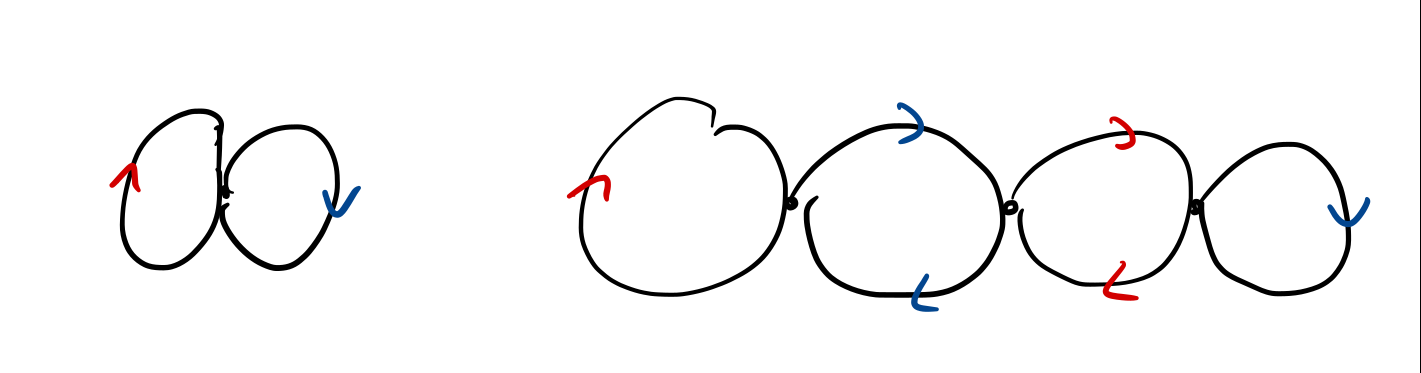
\includegraphics[scale=0.25]{figures/handdrawn/skizze-nach-19.3}
    \captionof{figure}{Eine Überlagerung von $S^1 \twedge S^1$}
\end{minipage}

Mit dem \autoref{thm:hauptsatz-der-überlagerungstheorie} ergibt sich nun der folgende Alternative Beweis:

\begin{proof}[Alternativer Beweis von \autoref{thm:isomorphismus-von-decktransformationen-mit-nebenklassengruppe-von-charakteristischer-untergruppe-in-seinem-normalisator}]
    
    Es sind $\Delta(p)$ genau die Automorphismen der Überlagerung  $p\colon  E \to X$. Nach dem Hauptsatz sind diese also isomorph zu den Automorphismen von $p^{-1} (x_0)$ als $\pi_1(X,x_0)$-Mengen, die wiederum isomorph sind zu den Automorphismen von $\cofaktor{p_*(\pi_1(E,e_0))}{\pi_1(X,x_0)}$, d.h.
\[
    \Delta(p) = \Aut \left(
    \begin{tikzcd}
        E \ar{d}{p} \\ X
    \end{tikzcd}\right) 
    \cong \Aut_{\pi_1(X,x_0)-\text{Mengen}} (p^{-1} (x_0)) \cong \Aut \left( \cofaktor{p_*(\pi_1(E,e_0)}{\pi_1(x,x_0)} \right) 
.\] 
\end{proof}

\begin{proposition}
    Es ist
    \[
        \Aut_{G-\text{Mengen}}\left(\cofaktor{H}{G}\right) \cong \cofaktor{H}{N_GH}
    .\] 
\end{proposition}
\begin{proof}
    Sei $f\colon  \cofaktor{H}{G} \to  \cofaktor{H}{G}\in \Aut \left(\cofaktor{H}{G}\right)$ ein solcher Automorphismus.
    \begin{enumerate}[1)]
    \item Dann ist $f$ bereits eindeutig bestimmt durch  $f(H)$ nach \autoref{lm:morphismus-von-g-mengen-von-transitiver-menge-ist-auf-einem-element-bestimmt}.
    \item $f(H.1) \in \cofaktor{H}{N_GH}$. ist $f(H.1) = H.g_0$, dann ist für alle $h\in H$ auch $H.g_0 = f(H.1) = f(H.h) = f(H.1).h = H.g_0.h$.

        Daraus folgt bereits, dass $\exists h_1,h_1 \in H$ mit $h_1g_0 = h_2g_0h$, also nach umformen
        \[
       h_2^{-1}h_1 = g_0hg_0^{-1}
        .\] 
        wegen $h\in H$ beliebig ergibt sich also bereits $g_0Hg_0^{-1}\subset H$. Das Inverse schickt $Hg_0$ auf $H$. Also schickt se  $H$ auf  $Hg_0^{-1}$. Analog zeigen wir, dass $g_0^{-1}Hg_0 \subset H$, also auch $H\subset g_0Hg_0^{-1}\subset H$ und somit schlussendlich
        \[
        H = g_0Hg_0^{-1} \qquad \implies \qquad g_0\in N_GH
        .\] 
        Die Abbildung
        \[
            f \mapsto f(H\cdot 1)
        .\] 
        ist also wohldefiniert und injektiv nach 1)

    \item Wir zeigen noch Surjektivität. Ist $g_0\in N_GH$, so behaupten wir, dass
        \[
        Hg \mapsto Hg_0g
        .\] 
        wohldefiniert und $G$-äquivariant ist. Die Äquivarianz ist nach Definition offensichtlich. Für Wohldefiniertheit bilden wir ab
         \[
             Hhg \mapsto H g_0hg \stackrel{g_0\in N_GH}{=} H h'g_0g = Hg_0g
        .\] 
        Da $N_GH$ eine Untergruppe ist, ist auch  $g_0^{-1}\in N_GH$, also hat die Abbildung ein Inverses, und zwar
        \[
        Hg \mapsto Hg_0^{-1}g
        .\] 
\end{enumerate}
\end{proof}

    % end lectures
\end{document}
